\chapter{Stage}
\label{ch:tesi:stage}

\section{Piano di stage}
\label{sec:tesi:stage:piano}

\subsection{Obiettivi e requisiti}
\label{sec:tesi:stage:piano:obiettivi}
L'attività di stage si colloca nell'ambito del progetto presentato nel capitolo \ref{ch:tesi:progetto} e persegue due obiettivi distinti ma correlati, focalizzandosi sulla componente \textit{social} della piattaforma.

\paragraph{Criteri di classificazione} \hfill \\
Il primo obiettivo consiste nell'estendere l'attuale sistema di classificazione (v. sezione \ref{sec:tesi:progetto:classificazione}) integrandovi un criterio aggiuntivo per la catalogazione dei contenuti pubblicati dagli utenti e la costruzione di un'enciclopedia della conoscenza per rendere il reperimento e la consultazione delle informazioni desiderate il più efficiente ed agevole possibile.

L'ideazione e concezione del suddetto criterio deve tener conto della natura tematica della piattaforma, riuscendo a conciliare due esigenze distinte:
\begin{itemize}
\item dev'essere sufficientemente astratto e flessibile per adattarsi alla molteplicità di varianti tematiche in cui la piattaforma stessa può essere declinata;
\item dev'essere ottimizzato per avvantaggiarsi delle peculiarità di una piattaforma tematica, ad esempio la maggior correlazione degli argomenti trattati.
\end{itemize}

La soluzione individuata deve inoltre prescindere da assunzioni legate alla tecnologia utilizzata. Infine, alla luce di possibili evoluzioni nello sviluppo della piattaforma, si desidera che la classificazione di un contenuto informativo (assegnazione di metadati, individuazione di correlazioni, \ldots) possa essere - in futuro - demandata a componenti software integrate nella piattaforma.

\paragraph{Interfaccia grafica} \hfill \\
Il secondo obiettivo consiste nel progettare un'interfaccia grafica per la consultazione dei contenuti informativi, che sfrutti il criterio di classificazione aggiuntivo per facilitare la ricerca ed il reperimento delle informazioni di interesse per l'utente all'interno del patrimonio enciclopedico della piattaforma. La sfida principale consiste nel progettare un'interfaccia in grado di visualizzare in maniera chiara e ordinata un ridotto o elevato numero di contenuti, a prescindere dalla classe del dispositivo impiegato (\textit{smartphone}, \textit{tablet}, \textit{notebook}, \ldots).

Il primo passo consiste nell'individuare le informazioni essenziali ad una rapida e precisa identificazione dei contenuti (titolo, autore, data, \ldots) e valutare la notazione (grafica o testuale) più adatta per esprimerle, al fine di renderle accessibili al maggior numero possibile di utenti; le informazioni aggiuntive devono essere comunque accessibili, ma solo su esplicita richiesta dell'utente. In questo ambito si inseriscono una serie di analisi e valutazioni di carattere sociologico, svolte da altri membri del team di progetto, per individuare le soluzioni più idonee a comunicare tali informazioni in modo da renderne la comprensione chiara e intuitiva a qualsiasi utente.

Il secondo passo richiede di definire le specifiche per un'interfaccia facilmente navigabile, che sia in grado di mostrare in modo ordinato e intuitivo i contenuti e le reciproche relazioni. Occorre perciò individuare opportuni criteri di raggruppamento, ordinamento e collocamento dei contenuti visualizzati per favorirne la consultazione, evitando un sovraccarico cognitivo e garantendo un livello adeguato di leggibilità.

Con il terzo ed ultimo passo si intende aggiungere la possibilità per l'utente di filtrare i contenuti visualizzati in accordo a proprietà (argomento, autore, data di pubblicazione, tipo) o metadati associati (attinenza, emozioni, giudizi, intenzioni). Per gli utenti autenticati si desidera offrire un livello aggiuntivo di personalizzazione, che consenta di filtrare automaticamente i contenuti secondo le preferenze associate al profilo (interessi, livello di esperienza).

Per individuare i requisiti essenziali si prendono innanzi tutto in considerazione alcuni casi d'uso classici:
\begin{enumerate}
\item l'utente naviga liberamente tra i contenuti (più recenti, più letti, più discussi, \ldots);
\item l'utente consulta la discussione generata da un singolo contenuto;
\item l'utente cerca le informazioni riguardanti un certo tema (contenuti affini, \ldots);
\item l'utente esplora gli argomenti trattati e le reciproche relazioni.
\end{enumerate}

\subsection{Pianificazione}
L'attività di stage viene suddivisa in due fasi distinte per semplificarne la pianificazione:
\begin{enumerate}
\item l'estensione del sistema di classificazione;
\item l'analisi e la progettazione dell'interfaccia grafica.
\end{enumerate}

Per ciascuna fase sono fissati gli obiettivi generali, sono individuate e organizzate su base settimanale le attività da svolgere, cercando di garantire un carico di lavoro equilibrato, e sono indicati i prodotti attesi. La durata complessiva dello stage si attesta su 8 settimane a tempo pieno, corrispondenti a 320 ore di lavoro.

\begin{table}[ht]
\centering
\begin{tabular}{|p{10cm}|c|}
\hline
\textsc{Attività} & \textsc{Ore di lavoro} \\ \hline
\multicolumn{2}{|c|}{\textit{Fase 1: estensione del sistema di classificazione}} \\ \hline 
Analisi delle specifiche del sistema di classificazione & 40 \\ \hline
Analisi comparativa dei principali sistemi di classificazione della conoscenza & 40 \\ \hline
Progettazione del sistema di classificazione & 40 \\ \hline
Implementazione del sistema di classificazione nel modello relazionale & 40 \\ \hline
\multicolumn{2}{|c|}{\textit{Fase 2: analisi e progettazione dell'interfaccia grafica}} \\ \hline 
Analisi dei requisiti dell'interfaccia grafica & 40 \\ \hline
Progettazione dell'interfaccia grafica: visualizzazione dei contenuti & 40 \\ \hline
Progettazione dell'interfaccia grafica: filtraggio dei contenuti & 40 \\ \hline
Progettazione dell'interfaccia grafica: navigazione dei contenuti & 40 \\ \hline
\end{tabular}
\caption{Pianificazione settimanale delle attività}
\label{tab:tesi:stage:pianificazione}
\end{table}

\begin{figure}[ht]
\begin{center}
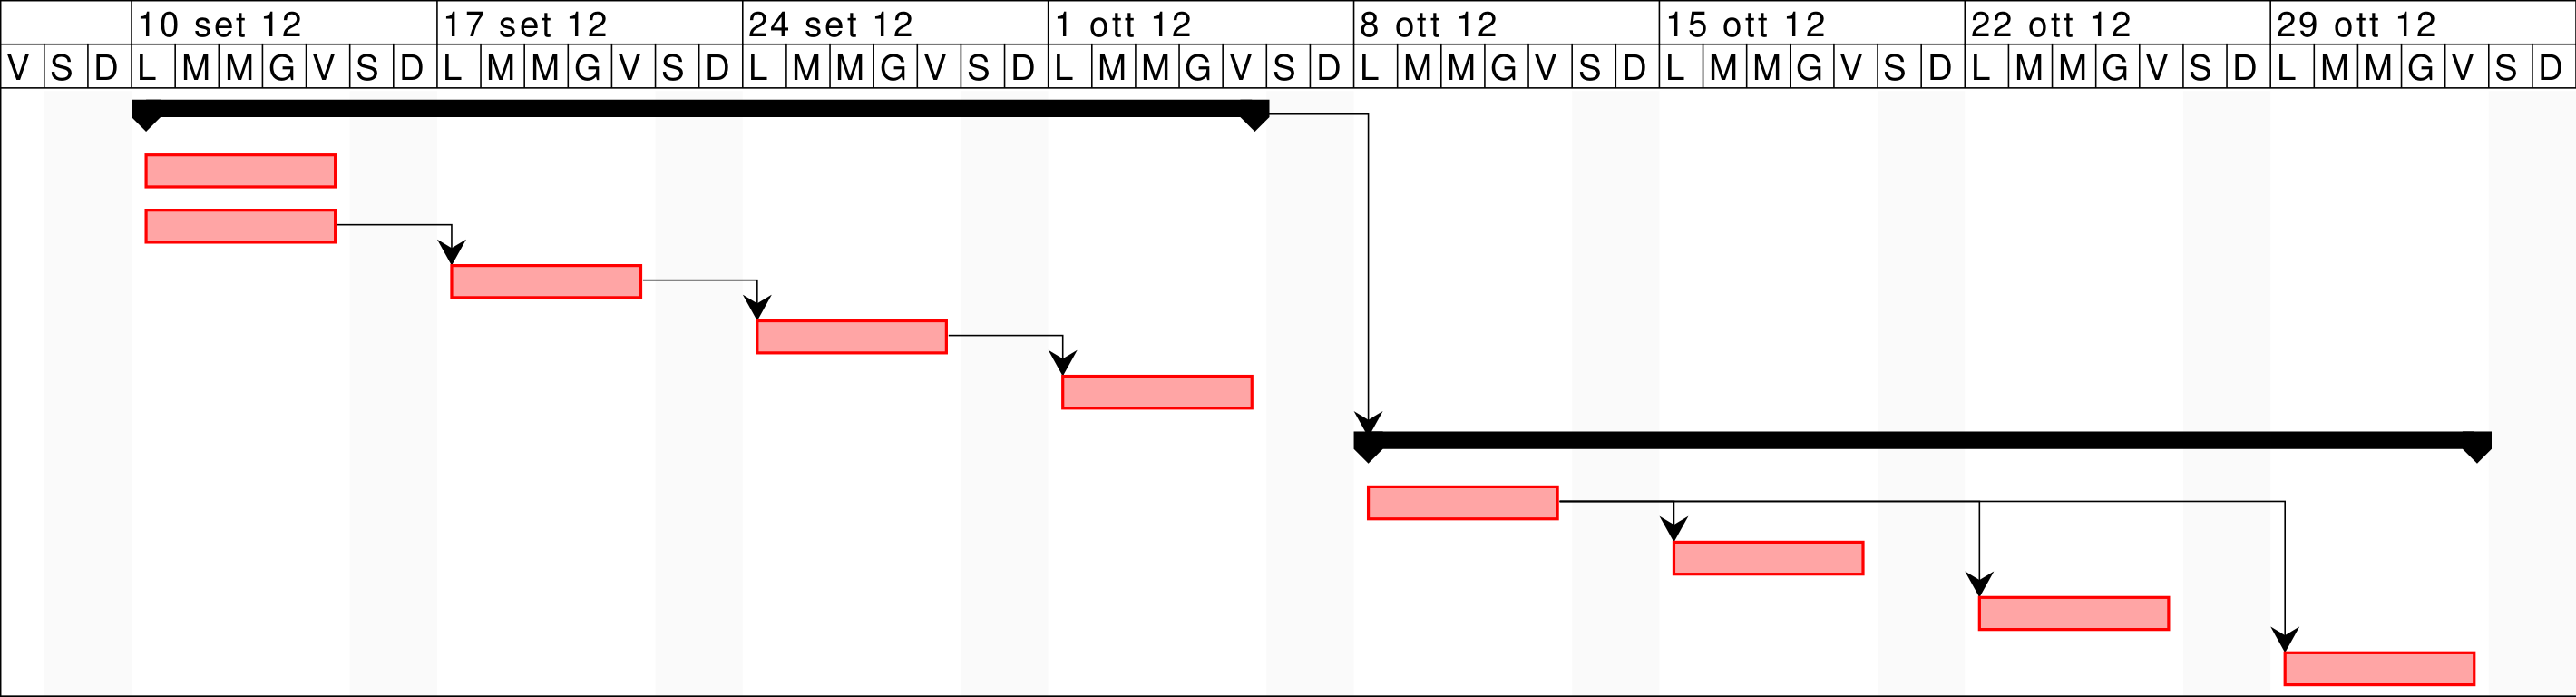
\includegraphics[width=14.5cm]{gantt.png}
\label{fig:tesi:stage:gantt}
\caption{Diagramma di Gantt}
\end{center}
\end{figure}

\section{Norme di stage}

\paragraph{Ambiente di lavoro}
Nel corso dello stage sono stati impiegati diversi strumenti per gestire le attività di progetto e produrre la documentazione prevista.

\begin{table}[ht]
\centering
\begin{tabular}{|l|l|}
\hline
\textsc{Controllo di versione} & \underline{Mercurial} 2.0.2 \\ \hline
\textsc{Editor \LaTeX} & \underline{LaTeXila} 2.4.0 - \underline{gedit} 3.4.0 con \textit{gedit-latex-plugin} \\ \hline
\textsc{Editor UML} & \underline{UMLet} 11.5.1 \\ \hline
\textsc{Foglio elettronico} & \underline{LibreOffice Calc} 3.6 \\ \hline
\textsc{Gestione database} & \underline{MySQL Workbench} 5.2.42 \\ \hline
\textsc{Mockup} & \underline{Pencil} 2.0.2 \\	\hline
\textsc{Pianificazione} & \underline{ProjectLibre} 1.5.1 \\ \hline
\textsc{Repository} & \underline{Bitbucket} \\ \hline
\textsc{Sistema operativo} & \underline{Ubuntu} 12.04 \\ \hline
\end{tabular}
\caption{Configurazione dell'ambiente di lavoro}
\label{tab:tesi:stage:norme:strumenti}
\end{table}

\paragraph{Documentazione}
La documentazione è stata redatta in \LaTeX\ e pubblicata in formato \underline{PDF}. A ciascun documento è assegnato un numero di versione $x.y$, ove $x$ rappresenta l'ultima \textsc{versione formale}, rivista e approvata dal referente aziendale e disponibile a terze parti interessate (membri del team di progetto, tutor interno), mentre il numero $y$ si riferisce ad una \textsc{versione preliminare} per uso interno, eventualmente consultabile dal referente aziendale.

\paragraph{Modello relazionale}
Il modello relazionale del database è stato realizzato mediante lo strumento adottato dal team di progetto, ossia l'editor \textit{MySQL Workbench}, per facilitare la condivisione e l'integrazione delle informazioni.

I nomi delle tabelle sono espressi in lingua italiana e contengono solo caratteri alfabetici minuscoli e non accentati, eventualmente separati mediante il simbolo '\textunderscore' (trattino basso). I nomi degli attributi, preceduti dal nome della tabella e dal carattere '.' (punto), sono espressi in lingua italiana e contengono solo caratteri alfabetici in formato \underline{CamelCase}, ove la lettera iniziale è sempre in minuscolo.

\paragraph{Digrammi UML}
Durante l'attività di stage sono stati redatti e inclusi nella documentazione diversi diagrammi \underline{UML} dei casi d'uso, dei package e delle classi, di cui sono presenti svariati esempi nel prosieguo del documento.

I nomi delle sottoclassi riportano per esteso o in forma abbreviata l'identificatore della superclasse diretta: nel secondo caso sono presenti - come prefisso - le sole lettere maiuscole, nel medesimo ordine di apparizione.

\paragraph{Casi d'uso}
La notazione utilizzata per identificare un caso d'uso è così definita:
$$UC.x.y$$
ove:
\begin{itemize}
\item $UC$ è l'abbreviazione di \textit{Use Case} (Caso d'uso);
\item $x \in \left\{1,2,\ldots\right\}$ è il numero identificativo del diagramma cui appartiene il caso d'uso;
\item $y \in \left\{1,2,\ldots\right\}$ è il numero associato al caso d'uso.
\end{itemize}

\paragraph{Requisiti funzionali}
I requisiti del sistema software sono univocamente identificati mediante la seguente notazione:
$$Rf.x.y$$
ove:
\begin{itemize}
\item $Rf$ è l'abbreviazione di \textit{requisito funzionale};
\item $x \in \left\{ob,de\right\}$ rappresenta il tipo di requisito funzionale (\textit{ob} per obbligatorio, \textit{de} per desiderabili);
\item $y \in \left\{1,2,\ldots\right\}$ è il numero associato ad un requisito.
\end{itemize}

\paragraph{Tracciamento dei casi d'uso}
Il tracciamento delle dipendenze tra casi d'uso e requisiti software è stato realizzato mediante un foglio elettronico, ove:
\begin{itemize}
\item ciascuna riga rappresenta un requisito del sistema software;
\item ciascuna colonna rappresenta un caso d'uso;
\item ciascuna cella contiene il carattere 'X' se esiste una relazione di dipendenza tra il caso d'uso e il requisito, altrimenti è vuota.
\end{itemize}

Per ciascuna riga e colonna viene impiegata una semplice formula per asserire la completezza e la necessità della matrice dei requisiti:  
\begin{center}
\texttt{CONTA.SE(A:Z;``X'')}   
\end{center}
ove:
\begin{itemize}
\item \texttt{A:Z} corrisponde all'intervallo di celle di una singola riga o colonna;
\item \texttt{"X"} rappresenta il pattern da cercare;
\item \texttt{CONTA.SE} è una funzione che accetta due argomenti (l'intervallo di celle ed il \textit{pattern}) e restituisce il numero di celle appartenenti all'intervallo contenenti una o più occorrenze del \textit{pattern} specificato.
\end{itemize}

\paragraph{Completezza} Per ogni colonna, se la formula restituisce un valore pari a 0 (zero) sta ad indicare che il requisito utente non è soddisfatto da alcun requisito software.

\paragraph{Necessità} Per ogni riga, se la formula restituisce un valore pari a 0 (zero) sta ad indicare che il requisito software corrispondente è superfluo.

%--------
% SECTION
%--------
\section{Criterio di classificazione}
\label{sec:tesi:stage:criterio-classificazione}
Il patrimonio di conoscenza della piattaforma è garantito essenzialmente dai contenuti pubblicati dagli utenti ed arricchito dal loro valore informativo: ciascuno di essi, a prescindere dalla forma (testo, immagini, audio, video, \ldots) o dalla classe (domanda, discorso, evento, recensione, \ldots), condivide delle informazioni inerenti uno o più elementi del dominio tematico della piattaforma.

\begin{figure}[ht]
\begin{center}
 
\includegraphics{placeholder.png}
 \label{fig:tesi:stage:classificazione:serbatoio-contenuti}
 \caption{Contenuti informativi e conoscenza}
\end{center}
\end{figure}

\paragraph{Contenuti informativi}
Allo state attuale, la piattaforma si limita ad essere un serbatoio di \textsc{contenuti informativi} disaggregati, priva degli strumenti per classificare e catalogare il sapere custodito conferendovi una struttura ordinata, una sorta di indice enciclopedico in grado di facilitarne la ricerca, il reperimento e la consultazione.

Ciascun contenuto rappresenta - dal punto di vista conoscitivo - una collezione di frammenti di informazioni, ciascuno dei quali contribuisce ad arricchire la conocenza relativa a qualche \textsc{entità}, oggetto di discussione all'interno del dominio della piattaforma.

\begin{figure}[ht]
\begin{center}
 
\includegraphics{placeholder.png}
 \label{fig:tesi:stage:fase-uno:contenuti-informativi}
 \caption{Valore informativo di un contenuto}
\end{center}
\end{figure}

\paragraph{Dominio conoscitivo}
L'insieme di entità definite - in un certo istante - all'interno della piattaforma ne costituisce il \textsc{dominio della conoscenza} (di seguito per brevità \textsc{dominio}), in maniera analoga a quanto accade con i lemmi di un'enciclopedia. Ciascun frammento di informazione presente in un contenuto è concettualmente associabile e riferibile ad una o più entità del dominio.

L'obiettivo primario del nuovo criterio di classificazione consiste dunque nel modellare tale dominio e le relazioni esistenti tra le entità ed i contenuti informativi.

\begin{figure}[ht]
\begin{center}
 
\includegraphics{placeholder.png}
 \label{fig:tesi:stage:fase-uno:dominio-conoscenza}
 \caption{Dominio di conoscenza della piattaforma}
\end{center}
\end{figure}

\subsection{Entità}  
Le \textsc{entità} $d_i \in D$ del dominio rappresentano elementi concreti (luoghi, persone, eventi, \ldots) o astratti (concetti, \ldots) a cui afferiscono i contenuti. Ciascuna di esse costituisce metaforicamente un lemma dell'enciclopedia del sapere disponibile presso la piattaforma e - pur avendo un preciso valore semantico - dev'essere identificata sul piano sintattico mediante un'\textsc{etichetta} $e_j \in E$.

%\begin{equation}
%e_j = f(d_i)
%\end{equation}

\paragraph{Ambiguità sintattica}
Gli utenti possono tuttavia riferirsi ad un'entità $d_i$ con termini o espressioni differenti ($e_{i,j} \in E_i$): tale ambiguità non può essere ignorata o trascurata e impone di considerare la relazione tra l'entità e le etichette con cui può essere riferita di tipo uno-a-molti. Il criterio di classificazione dev'essere quindi in grado di esprimere il fatto che tali etichette rappresentino sinomini di una stessa entità.

\begin{figure}[ht]
\begin{center}

\includegraphics{placeholder.png}
\label{fig:tesi:stage:fase-uno:ambiguita-sintattica-entita}
\caption{Ambiguità sintattica di un'entità}
\end{center}
\end{figure}

\paragraph{Etichette duplicate}
Allo stesso tempo occorre impedire la proliferazione di etichette duplicate, ossia equivalenti sul piano semantico ma sintatticamente differenti. Un fenomeno simile avrebbe inevitabili ripercussioni sull'efficacia del criterio di classificazione e sull'efficienza della ricerca: reperire tutte e sole le informazioni inerenti una certa entità richiederebbe infatti di individuare tutte le etichette con cui possa essere riferita e cercare riscontri per ciascuna di esse nei contenuti pubblicati.

Per incrementare l'efficienza di catalogazione e ricerca dei contenuti risulta conveniente che l'entità sia identificata univocamente nei contenuti informativi, a prescindere dalla specifica etichetta utilizzata.

\paragraph{Sintassi e semantica}
Il fattore essenziale consiste nel mantenere separata la componente semantica (il dominio delle entità) da quella sintattica (il dizionario delle etichette): solo così è possibile stabilire un associazione naturale e diretta tra i contenuti e le entità, a prescindere dalle etichette.

\begin{figure}[ht]
\begin{center}

\includegraphics{placeholder.png}
\label{fig:tesi:stage:fase-uno:entita-sintassi-semantica}
\caption{Sintassi e semantica di un'entità}
\end{center}
\end{figure}

Ciò non toglie la necessità di individuare un'etichetta, che permetta di esprimere e comunicare l'entità cui si fa riferimento: per soddisfare tale condizione si individua - per ciascuna entità - un'\textsc{etichetta primaria} $e_{i,0}$, che la identifica univocamente nell'ambito della piattaforma, mentre le restanti (\textsc{etichette secondarie}) ne vengono considerate sinonimi.

%\begin{equation}
%e_{i,0} = f'(d_i)
%\end{equation}

\paragraph{Relazioni}
Riprendendo la metafora enciclipedica, ciascun lemma contiene spesso riferimenti ad altre voci, che trattano temi specifici o attinenti: ci si aspetta che tali relazioni siano replicabili anche nel dominio della piattaforma sotto forma di legami molti-a-molti tra le entità.

\begin{figure}[ht]
\begin{center}

\includegraphics{placeholder.png}
\label{fig:tesi:stage:fase-uno:entita-relazioni}
\caption{Relazioni tra entità}
\end{center}
\end{figure}

A questo punto il dominio può essere intepretato come un grafo orientato ove:
\begin{itemize}
\item ciascun nodo rappresenta un entità, identificata dalla relativa etichetta primaria;
\item ciascun arco uscente identifica un'entità riferita;
\item ciascun arco uscente identifica un'entità referente.
\end{itemize}

\subsection{Etichette}
Un'\textsc{etichetta} $e_j \in E$ rappresenta la forma sintattica - una stringa di lunghezza variabile - mediante la quale gli utenti ed il sistema identificano un'entità del dominio. L'insieme di etichette definite in un certo istante costituisce il \textsc{dizionario} della piattaforma.

\paragraph{Accezioni}
Analogamente ad un lemma enciclopedico, un'etichetta può risultare semanticamente ambigua ed essere caratterizzata da svariate \textsc{accezioni} $a_{j,k} \in A_j$, ciascuna delle quali assume un significato e si riferisce ad un'entità distinti. Da questa prospettiva, la natura tematica della piattaforma dovrebbe contribuire a limitare il numero medio di accezioni per ciascuna etichetta.

\begin{figure}[ht]
\begin{center}

\includegraphics{placeholder.png}
\label{fig:tesi:stage:fase-uno:etichette-accezioni}
\caption{Accezioni di un'etichetta}
\end{center}
\end{figure}

L'etichetta $e_j$ identifica dunque entità del dominio distinte, a seconda dell'accezione $a_{j,k}$ considerata: la distinzione tra etichetta primaria e secondaria si trasferisce dunque alle accezioni, che si distinguono in \textsc{chiave} o \textsc{sinonimica}.

\begin{description}
	\item[Accezione chiave] \hfill \\
	L'accezione chiave $a_{j,0}$ indica che la relativa etichetta $e_j$ identifica univocamente l'entità corrispondente: ciò significa che - in ogni istante - a ciascuna entità dev'essere associata una e una sola etichetta primaria. Qualora si rimuova un'accezione chiave di un'etichetta, occorre individuare una nuova etichetta primaria per l'entità riferita.
	\item[Accezione sinonimica] \hfill \\
	L'accezione sinonimica ($a_{j,1},\ldots,a_{j,\left|A_j\right|}$) indica che l'etichetta associata $e_j$ rappresenta un sinonimo dell'entità corrispondente. La relazione uno-a-molti tra entità ed etichette si traduce dunque in:
	\begin{itemize}
		\item una relazione uno-a-molti tra le etichette e le accezioni:
		%\begin{equation}
		%e_j = g(a_{j,k})
		%\end{equation}
		\item una relazione uno-a-molti tra le entità e le accezioni:
		%\begin{equation}
		%d_i = h(a_{j,k})
		%\end{equation}
	\end{itemize}
\end{description}

\paragraph{Sinonimi}
Sebbene le entità siano identificate univocamente dalle corrispondenti etichette primarie, è assai utile includere e conservare nel dizionario anche i sinonimi (etichette secondarie) note o utilizzate dagli utenti al fine di garantire maggiore copertura sintattica, aumentando così la probabilità che i termini o le espressioni utilizzati successivamente per riferire una certa entità siano gia presenti nel dizionario e quindi immediatamente riconoscibili.

\paragraph{Ricerca}
L'utente alla ricerca di informazioni riguardanti un particolare tema cerca in genere le etichette che presentino maggior attinenza. Per evitare la proliferazione di etichette semanticamente identiche e sintatticamente simili, si fissa uno standard per il formato, che normi la capitalizzazione delle lettere, la gestione degli spazi, \ldots al fine di uniformare la struttura sintattica delle etichette.

L’osservanza e l’adesione a tali regole da parte delle etichette inserite viene accertata automaticamente, provvedendo - ove necessario - ad apportare le opportune correzioni per adeguarle allo standard, e rappresenta un requisito essenziale per garantire la consistenza del dizionario della piattaforma.

\subsection{Contenuti}  
L'obiettivo primario del criterio di classificazione consiste nel tenere traccia delle entità riferite all'interno di ciascun contenuto per rendere facilmente reperibili le informazioni che le riguardano.

\paragraph{Valore informativo}
Ciascun contenuto reca con sé informazioni riguardanti una o più entità: ne consegue che la relazione tra entità e contenuti sia di tipo molti-a-molti (\texttt{n:m}). Preservare la distinzione tra entità (semantica) ed etichette (sintassi) consente di identificare in maniera chiara e univoca nell'intera piattaforma ciò a cui si fa riferimento nei vari contenuti, a prescindere dai termini o dalle espressioni linguistiche impiegati per indicarli.

\paragraph{Catalogazione}
L'assegnazione di un'etichetta ad un contenuto è un processo che traduce un ingresso sintattico dell'utente (l'etichetta) in un'uscita semantica (l'entità), che viene effettivamente e concretamente assegnata al contenuto.

Sebbene si sia scelto di riferire - nei contenuti pubblicati - ciascuna entità sempre e solo con l'etichetta primaria, per ragioni di semplicità ed efficienza (l'etichetta primaria è un'informazione strettamente correlata all'entità), nulla impedirebbe di assegnare ai contenuti qualsiasi etichetta scelta dagli utenti. Ciò comporterebbe tuttavia la necessità di associare al contenuto non solo l'entità, ma anche - tra le possibili - l'etichetta scelta per indicarla.

\subsection{Utente}
Le scelte progettuali descritte nelle sezioni precedenti sono state valutate tenendo presenti alcuni casi d'uso inerenti l'esplorazione dei contenuti pubblicati nella piattaforma da parte dell'utente, arrivando a delinarne alcuni di particolare interesse o rilevanza. La metafora dell'enciclopedia, che accosta il nuovo criterio di classificazione ad un indice enciclopedico, esprime in maniera assai accurata e favorisce la comprensione delle dinamiche e degli obiettivi con cui gli utenti consultano il sapere della piattaforma. 

\paragraph{Ricerca per temi}
La ricerca per temi consiste essenzialmente in un'esplorazione dei contenuti informativi a partire dalle entità, che sono assimilabili agli argomenti di discussione, in maniera analoga alla consultazione dei un'enciclopedia, quando si procede da un lemma all'altro, facendosi guidare dai riferimenti tra le voci sino a trovare quella di interesse. Nella piattaforma ciò si esprime in un'esplorazione libera del grafo orientato delle entità, ciascuna identificata dalla relativa etichetta primaria.

\paragraph{Ricerca per etichette}
La classica strategia di ricerca prevede l'inserimento di alcune parole chiave, che agli occhi dell'utente identificano l'informazione cui è interessato e hanno maggiore probabilità di essere associate o comparire nei contenuti.

Nella piattaforma, una volta riconosciuta un'etichetta in un termine inserito, occorre identificare il valore semantico (l'entità) attribuitole dall'utente, inevitabilmente associato ad un'accezione dell'etichetta stessa, così da giungere ad identificare univocamente l'entità cercata.

Ove la ricerca si soffermi a considerare l’etichetta, i risultati possono risultare parziali, includendo i soli contenuti in cui l’entità sia riferita dalla specifica etichetta, o addirittura non pertitenti, includendo contenuti ove l'etichetta è presente ma in un'accezione differente.

Un ulteriore aspetto da considerare riguarda la dimensione del dizionario $E$ e del dominio $D$: sapendo che ciascuna accezione rappresenta una coppia <etichetta,entità> univoca, possiamo esprimere il numero medio di etichette associate a ciascuna entità come:
\begin{equation}
\alpha = \frac{\sum{\left|A_j\right|}}{\left|D\right|}
\end{equation}
Assegnando ai contenuti un'etichetta qualsiasi si aumenterebbe di una costante moltiplicativa $\alpha$ la complessità dell'operazione ricerca, dovendola ripetere per ciascuna delle $\alpha$ etichette anziché per la sola entità corrispondente.\footnote{Si assuma per semplicità che la ricerca verifichi - per ciascun contenuto - quali termini cercati (entità o etichette) siano presenti, uno per volta, e che la complessità computazionale sia equivalente in entrambi i casi.}

La rilevanza di un contenuto informativo rispetto ai criteri di ricerca è infine determinata dal grado di corrispondenza rispetto alle entità cercate: maggiore è il numero di riscontri, maggiore sarà approssimativamente la rilevanza attribuita nel contesto della ricerca.

Se $E_s$ è l'insieme delle etichette cercate e $E_c$ l'insieme delle etichette assegnate a ciascun contenuto si possono distinguere tre casi principali:
\begin{description}
\item[Corrispondenza completa:] $E_s \subseteq E_c$ \hfill \\
Al contenuto risultano assegnate tutte le entità cercate (massima attinenza).
\item[Corrispondenza parziale:] $E_s \cap E_c \neq \emptyset$ \hfill \\
Al contenuto risulta assegnata parte delle entità cercate (media attinenza).
\item[Nessuna corrispondenza:] $E_s \cap E_c = \emptyset$\hfill \\
Al contenuto non risulta assegnata alcuna entità cercata (attinenza nulla).
\end{description}

\paragraph{Ricerca per affinità}
Il terzo approccio di ricerca consiste nell'identificare i contenuti attinenti ad uno dato, ossia aventi il maggior numero di entità in comune. Valgono per questo scenario le medesime considerazioni fatte nella sezione precedente, previa sostituzione di $E_s$ con l'insieme delle etichette assegnate al contenuto corrente.

\subsection{Modello relazionale}

\begin{figure}[ht]
\begin{center}
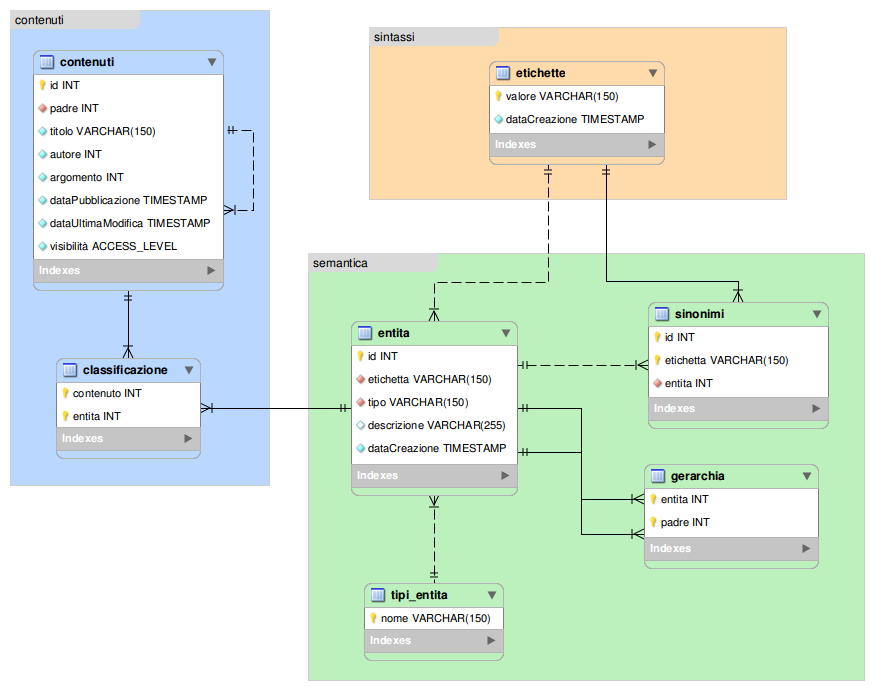
\includegraphics[width=14.7cm]{modello-er.png}
\label{fig:tesi:stage:er:modello}
\caption{Modello relazione del criterio di classificazione}
\end{center}
\end{figure}

Al termine della fase progettuale, si rende necessario aggiungere al modello relazionale della piattaforma le opportune modifiche per integrare le informazioni addizionali legate al nuovo criterio di classificazione.

Rispetto all'immagine \ref{fig:tesi:stage:er:modello}, la sola tabella \textsf{contenuti} risulta importata dal modello relazionale della piattaforma per evidenziare alcune relazioni fondamentali. Le rimanenti sono organizzate in tre \textit{layer} (\textsf{contenuti}, \textsf{semantica} e \textsf{sintassi}) per chiarirne il ruolo all'interno del sistema di classificazione.

\paragraph{Entità}
Le entità vengono rappresentate mediante la tabella \textsf{entita} e si caratterizzano per due vincoli referenziali:
\begin{description}
\item[tipo] 
Chiave esterna verso la tabella \textsf{tipi\textunderscore entita}, indica se si tratti di luogo, evento, persona, concetto astratto, \ldots. 
\item[etichetta]
Chiave esterna verso la tabella \textsf{etichette}, rappresenta l'etichetta primaria associata all'entità.
\end{description}

La relazione di tipo molti-a-molti tra le entità si traduce nella tabella \textsf{gerarchia}, che contiene due chiavi esterne verso la medesima tabella \textsf{entita} a rappresentare rispettivamente le entità riferite e quelle referenti.

\paragraph{Etichette}
Le etichette sono rappresentate mediante la tabella \textsf{etichette} e sono identificate univocamente dalla stringa associata, che rappresenta l'attributo \textsf{etichette.valore}. Tale scelta risponde alla naturale identificazione dell'etichetta nella sequenza di caratteri corrispondente, costituisce una garanzia contro la presenza di duplicati e consente di recuperare il valore dell'etichetta primaria di un'entità senza dover effettuare un'operazione di \textit{join} tra le tabelle \textsf{entita} ed \textsf{etichette}.

\paragraph{Accezioni}
Le accezioni rappresentano un legame univoco tra le etichette e le entità e possono essere di tipo chiave o sinonimico. Esse non presentano attributi propri significativi, ma prevedono tre vincoli referenziali:
\begin{enumerate}
\item a ciascuna entità è associata una e una sola \textsc{accezione chiave} (relazione uno-a-uno), che identifica l'etichetta primaria;
\item a ciascuna entità sono associate $0\ldots n$ \textsc{accezioni sinonimiche} (relazione uno-a-molti), che rappresentano i sinonimi dell'etichetta primaria;
\item ciascuna etichetta possiede $0\ldots n$ \textsc{accezioni} (relazione uno-a-molti).
\end{enumerate}

\begin{figure}[ht]
\begin{center}

\includegraphics{placeholder.png}
\label{fig:tesi:stage:er:accezioni}
\caption{Modello ad oggetti delle accezioni}
\end{center}
\end{figure}

Ne consegue che sia la superclasse (\textsf{accezioni}) sia le sottoclassi (\textsf{accezioni\textunderscore chiave} e \textsf{accezioni\textunderscore sinonimiche}) presentano dei vincoli referenziali; in particolare, la presenza delle prime due relazioni costringe a distinguere - dal punto di vista dell'entità - tra accezioni chiave e sinonimiche.

Per modellare tale scenario vengono presi in considerazione tre possibili approcci:
\begin{description}
\item[Tabella unica] \hfill \\
La tabella unica ben si adatta a gestire l'assenza di attributi propri per le sottoclassi e ad esprimere i vincoli referenziali che coinvolgono la superclasse, ma non è in grado di esprimere e adeguatamente rappresentare quelli coinvolgenti le sottoclassi.
\item[Partizionamento orizzontale] \hfill \\
Il partizionamento orizzontale riesce a modellare i vincoli referenziali delle sottoclassi, ma non quello della superclasse, e genera due classi aventi i medesimi attributi.
\item[Partizionamento verticale] \hfill \\
Il partizionamento verticale consente di modellare correttamente tutti e tre i vincoli referenziali, relativi sia alla superclasse sia alle sottoclassi. Tuttavia si rende più complesso modificare il tipo di un'accezione e si introduce l'esigenza di un'operazione \textit{join} per recuperare la lista completa delle accezioni, pur non possedendo le sottoclassi attributi propri.
\end{description}

A seguito di alcune osservazioni si decide di adottare la soluzione della tabella unica:
\begin{itemize}
\item la distinzione tra etichette chiave e sinomimiche ha rilevanza essenzialmente dal punto di vista della classe \textsf{entita};
\item il vincolo referenziale tra \textsf{etichette} ed \textsf{accezioni} suggerisce che la distinzione di cui al punto precedente sia irrilevante dal punto di vista delle etichette, ragion per cui risulta utile mantenere tutte le accezioni nella medesima tabella.\footnote{Si consideri ad esempio il caso d'uso della ricerca di un'entità a partire da un'etichetta, ove occorre recuperare la lista completa delle relative accezioni.}
\item le sottoclassi non hanno attributi propri, per cui il partizionamento verticale e orizzontale sono da ritenersi soluzioni inadeguate o carenti.
\end{itemize}

Il soddisfacimento delle condizioni richieste viene raggiunto eliminando qualsiasi riferimento al tipo dell'accezione nella classe \textsf{accezioni} e modellando la relazione uno-a-uno tra le entita e le relative etichette primarie mediante una vincolo referenziale di chiave esterna nella classe \textsf{entita}, ossia \textsf{entita.etichetta}, che identifica la corrispondente etichetta primaria nella tabella \textsf{etichette}. Così facendo si riescono ad esprimere tutti i vincoli referenziali senza dover definire le sottoclassi.

\paragraph{Contenuti}
Il vincolo referenziale tra i contenuti e le entità rappresenta l'essenza del criterio di classificazione, consentendo di classificare e catalogare le informazioni disponibili nella piattaforma. La relazione molti-a-molti tra \textsf{contenuti} ed \textsf{entita} viene modellata aggiungendo la nuova classe \textsf{classificazione}, che tiene precisamente traccia delle entità associate a ciascun contenuto.

%--------
% SECTION
%--------
\section{Interfaccia grafica}
\label{sec:tesi:stage:gui}
La seconda fase dell'attività di stage consiste nell'analisi e nella progettazione di un'interfaccia grafica per la consultazione dei risultati di ricerche sui contenuti informativi, che soddisfi adeguatamente i seguenti requisiti di qualità:
\begin{description}
	\item[Intuitiva] \hfill \\
	L'interfaccia grafica deve risultare agevole e facilmente utilizzabile da qualsiasi categoria di utenti, a prescindere dal livello di esperienza e dalla familiarità con piattaforme web esistenti (\textit{chat}, \textit{forum}, \textit{social network}, \ldots).
	\item[Multipiattaforma] \hfill \\
	L'interfaccia grafica dev'essere fruibile dal maggior numero possibile di dispositivi (\textit{computer}, \textit{tablet}, \textit{smartphone}, \ldots), avendo ben presente le differenti modalità di interazione.
	\item[Ordinata] \hfill \\
	L'interfaccia grafica dev'essere in grado di rappresentare in maniera ordinata ed efficace le informazioni, a prescindere dal numero di contenuti caricati: quelle essenziali devono essere immediatamente disponibili e facilmente identificabili, mentre quelle aggiuntive o accessorie devono essere comodamente accessibili.
\end{description}

Per semplificare le fasi di analisi e progettazione il modello concettuale del prodotto software è stato suddiviso in tre componenti:
\begin{description}
 	\item[Ricerca] \hfill \\
 	Insieme dei parametri e criteri di ricerca (parole chiave, ambito di ricerca, \ldots).
 	\item[Filtri] \hfill \\
 	Insieme dei filtri di raffinamento della ricerca.
 	\item[Contenuti] \hfill \\
 	Insieme dei contenuti informativi corrispondenti ai criteri di ricerca.
 \end{description}
 
\paragraph{Obiettivi}
Le finalità d'interazione dell'utente con l'interfaccia grafica sono in buona parte riconducibili alla scomposizione concettuale del sistema, illustrata nella sezione precedente:
\begin{enumerate}
	\item impostare i parametri iniziali di ricerca o modificarli a posteriori;
	\item filtrare i risultati di ricerca in accordo a criteri di classificazione (argomento, emozione, etichetta, giudizio, intenzione, interessi) o proprietà dei contenuti (autore, data di pubblicazione, tipo);
	\item individuare i contenuti di interesse e consultare le informazioni associate;
	\item mostrare la discussione associata ad un contenuto informativo;
	\item impostare i filtri personalizzati (solo per utenti autenticati).
	\item rappresentare - in forma grafica o testuale - le proprietà fondamentali di ciascun contenuto (\ldots), i metadati di classificazione (emozioni, giudizi, intenzioni, \ldots) e i legami reciproci;
\end{enumerate}
 
\subsection{Risultati di ricerca}
\begin{enumerate}
	\item aggiornamento risultati a fronte
\end{enumerate}
- discussione
\paragraph{UC.1 - Ricerca di contenuti informativi} \hfill \\
La ricerca di contenuti informativi prevede l'inserimento dei termini di ricerca (\textit{UC.1.1}), separati da virgola, e la restrizione dell'ambito alle sole entità associate o alle informazioni presenti in un contenuto (titolo, corpo, \ldots) (\textit{UC.1.2}).

Durante la ricerca, qualora vengano individuate delle corrispondenze tra i termini cercati e le etichette del dizionario e queste presentino accezioni multiple, l'utente è chiamato a selezionare quella corrispondente all'entità rispetto alla quale intende svolgere la ricerca (\textit{UC.1.3}).

Al termine della ricerca, l'utente può consultare la lista delle entità individuate a partire dai criteri di ricerca specificati (\textit{UC.1.4}) e intervenire sui risultati di ricerca eliminando una di esse (\textit{UC.1.5}) o sostituendola con un'altra, avente un legame diretto (\textit{UC.1.8}, \textit{UC.1.9}). Per sostituire un'entità con un'altra l'attore dev'essere in grado di visualizzare - per ciascuna - quelle che la riferiscono (\textit{UC.1.6}) o da lei riferite (\textit{UC.1.7}).
 
\subsection{Filtri di ricerca}

\paragraph{UC.2 - Raffinamento dei criteri di ricerca} \hfill \\
Per facilitare l'individuazione dei contenuti di interesse tra i risultati dai ricerca, l'utente dev'essere messo in condizione di filtrarli ...

Il primo passo consiste nell'individuare le proprietà dei contenuti informativi aventi particolare rilevanza e definite su un insieme $U$ di valori adeguato ad essere associato ad un filtro: il solo requisito è la possibilità di partizionare l'insieme $U$ in due sottoinsiemi, che rappresentano rispettivamente i valori autorizzati ($U_a$) e bloccati ($U_b$) in un certo istante.

%Se consideriamo $U = U_a \cup U_b$

La configurazione predefinita di ciascun filtro prevede che tutti i valori siano ammissibili, ossia $U_a = U$ e $U_b = \emptyset$. L'azione dell'utente consiste essenzialmente nell'alterare tale partizionamento dell'insieme $U$ in tre modi principali:
\begin{itemize}
	\item bloccando un valore $u$ ($u \in U_b$);
	\item autorizzando un valore ($u \in U_a$);
	\item azzerando il filtro, ossia ripristinando la configurazione iniziale e autorizzando tutti i valori ($U = U_a$).
\end{itemize}

\begin{itemize}
	\item quali criteri di classificazione? quali proprietà ?
	\item classificazione
\end{itemize}

\paragraph{UC.4 - Gestione dei filtri utente}

\paragraph{Utente autenticato}
Nell'ambito dei filtri riservati all'utente autenticato l'individuazione, la classificazione e l'analisi dei casi d'uso inizia dal riconoscimento di due attori principali, ossia l'\textsc{utente autenticato} ed il visitatore (di seguito semplicemente \textsc{utente}. L'utente autenticato rappresenta un tipo specializzato del visitatore, dal momento che alcune informazioni di profilo, come gli interessi dichiarati o il livello di esperienza, vengono sfruttate per filtrare automaticamente i risultati di ricerca: a lui solo, dunque, è offerta la possibilità di abilitare o meno tali filtri personalizzati.

\subsection{Navigazione dei contenuti}
- discussione

\paragraph{UC.3 - Consultazione dei risultati di ricerca}
